
\providecommand{\Fun}{\operatorname{Fun}}
\providecommand{\Cat}{\mathcal{C}at}
\providecommand{\sSet}{s\mathcal{S}et}
\providecommand{\QCat}{\mathcal{Q}\mathcal{C}at}
\providecommand{\Set}{\mathcal{S}et}
\providecommand{\qcInt}{\mathbb{I}}   %
\providecommand{\CSS}{\mathcal{C}\mathcal{S}\mathcal{S}}
\providecommand{\Segal}{\mathcal{S}egal}
\providecommand{\PCat}{\mathcal{P}\mathcal{C}at}
\providecommand{\OneComp}{1\text{-}\mathcal{C}omp}
\providecommand{\rvDisc}{\mathrm{disc}}
\providecommand{\rvNerve}{\mathrm{nerve}}
\providecommand{\rvLan}{\mathrm{lan}}
\providecommand{\rvRan}{\mathrm{ran}}
\providecommand{\rvDiag}{\mathrm{diag}}

\section{\texorpdfstring{$(\infty,1)$}{(∞,1)}-\trCategory{}的%
\trInfinityCosmos}\label{sec:infinity-cosmoi-of-infinity-1-categories}

\trQuasiCategory{}的\trInfinityCosmos{}已在第 1 章中的%
\cref{prop:cosmos-quasi-categories}中得到确立。在本节中，我们将确立另外三座%
\trInfinityCosmos，其对象定义 $(\infty,1)$-\trCategory——分别以%
\trCompleteSegalSpaces、\trSegalCategories{}或 $1$-复状\trSimplicialSet{}为%
模型——并在它们之间构造下列\trBiequivalence：
\begin{center}
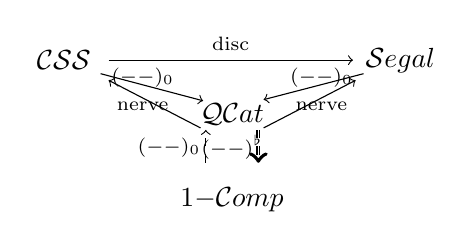
\begin{tikzpicture}[x=1.9em,y=1.4em]
  \node (css)   at (0,2.1)    {$\CSS$};
  \node (segal) at (6.4,2.1)  {$\Segal$};
  \node (qcat)  at (3.2,0.7)  {$\QCat$};
  \node (comp)  at (3.2,-1.5) {$\OneComp$};
  \draw[->] (0.85,2.1) -- node[above]{$\scriptstyle\rvDisc$} (5.5,2.1);
  \draw[->] (0.7,1.75) -- (2.65,1.05);
  \node at (1.5,1.66) {$\scriptstyle(\text{--})_{0}$};
  \draw[->] (2.6,0.35) -- (0.85,1.58);
  \node at (1.5,0.9) {$\scriptstyle\rvNerve$};
  \draw[->] (3.8,0.35) -- (5.55,1.58);
  \node at (4.9,0.9) {$\scriptstyle\rvNerve$};
  \draw[->] (5.7,1.75) -- (3.8,1.08);
  \node at (4.9,1.66) {$\scriptstyle(\text{--})_{0}$};
  \draw[->,dashed] (2.7,-0.55) -- (2.7,0.3);
  \node at (2.0,-0.15) {$\scriptstyle(\text{--})_{0}$};
  \draw[->,dashed,double] (3.7,0.3) -- (3.7,-0.55);
  \node at (3.2,-0.15) {$\scriptstyle(\text{--})^{\flat}$};
\end{tikzpicture}
\end{center}
在给出 Charles Rezk 在 \cite{bib100} 中引入的\trCompleteSegalSpaces{}之形式%
定义之前，我们先解释这一想法。首先，一个\trCompleteSegalSpaces{}是一个%
\textbf{双单纯集}（bisimplicial set）%
$X\in\Set^{\Delta^{\mathrm{op}}\times\Delta^{\mathrm{op}}}$。惯常的做法，是把诸单纯集%
$X_{m\bullet}\coloneqq X_{m,\bullet}$ 视作双单纯集 $X$ 的「列」，而诸单纯集 $X_{\bullet,n}$ 则定义%
「行」。在一个\trCompleteSegalSpaces{}中，如下\trDiagram
\[
X_{\bullet}\coloneqq X_{0}
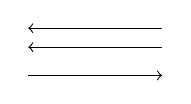
\begin{tikzpicture}[baseline=-0.5ex]
  \draw[<-] (0,0.30) -- (1.7,0.30);
  \draw[<-] (0,0.06) -- (1.7,0.06);
  \draw[->] (0,-0.30) -- (1.7,-0.30);
\end{tikzpicture}
X_{1}
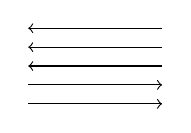
\begin{tikzpicture}[baseline=-0.5ex]
  \draw[<-] (0,0.42) -- (1.7,0.42);
  \draw[<-] (0,0.18) -- (1.7,0.18);
  \draw[<-] (0,-0.06) -- (1.7,-0.06);
  \draw[->] (0,-0.30) -- (1.7,-0.30);
  \draw[->] (0,-0.54) -- (1.7,-0.54);
\end{tikzpicture}
X_{2}\qquad\cdots
\]
定义 Kan 复形的\trCategory{}中的一个\trSimplicialObject。此外，对每个
$m\ge 0$，其余定义域是与该 $m$-\trSimplex{}相伴的「边界数据」之空间的匹配%
映射 $X_{m}\to M_{m}X$ 是一个\trKanFibration。诸空间 $X_{0}$ 与 $X_{1}$ 是%
\trCompleteSegalSpaces{}的「对象与箭头之空间」。所谓的「Segal 条件」蕴含：
空间 $X_{n}$ 可以被视作「$n$-可复合箭头之空间」。一个满足至此所列诸条件的
Segal 空间，便近乎某种「同伦意义上的内范畴」（与附录 B 中的%
\cref{def:internal-category}相比较）。最后一项「完全性」条件把 $X_{0}$ 的
空间性结构与刚刚定义的范畴性结构联系起来，表达了这样一种想法：$X_{0}$ 中的
路径应当对应于 $X_{\bullet}$ 中的诸\trIsomorphism。

\trCompleteSegalSpaces{}的形式定义有三项条件，用\trWeightedLimit{}%
\trBifunctor{}来描述它们最为容易：
\[
(\Set^{\Delta^{\mathrm{op}}})^{\mathrm{op}}\times \sSet^{\Delta^{\mathrm{op}}}
\xrightarrow{\ \operatorname{lim}_{-,-}\ }\sSet
\]
其中 $\sSet$ 被视作一个 $\Set$-富集的\trCategory。注意，$\sSet$ 中
$\Delta^{\mathrm{op}}$-索引之\trDiagram{}的诸权重乃是 $\Set$ 中的
$\Delta^{\mathrm{op}}$-索引之\trDiagram，亦即诸\trSimplicialSet。更为详细地：

\begin{definition}[完全 Segal 空间]\label{def:complete-segal-space}
\begin{enumerate}[label=(\roman*)]
\item 一个\trSimplicialObject{} $X_{\bullet}\in\sSet^{\Delta^{\mathrm{op}}}$
  是\textbf{Reedy 纤维性}的（Reedy fibrant），恰当其在加权极限上诱导的映射
  \[
  X_{m}\cong\operatorname{lim}_{\Delta[m]}X\longrightarrow
  \operatorname{lim}_{\partial\Delta[m]}X=:\ M_{m}X
  \]
  对一切 $m\ge 0$ 都是单纯集之间的\trKanFibration。
\item 一个 Reedy 纤维性的\trSimplicialObject{} $X_{\bullet}$ 是一个%
  \textbf{Segal 空间}（Segal space），恰当其在加权极限上诱导的映射
  \[
  X_{n}\cong\operatorname{lim}_{\Delta[n]}X\longrightarrow
  \operatorname{lim}_{\Lambda^{k}[n]}X
  \]
  对一切 $n\ge 2$ 与 $0<k<n$ 都是单纯集之间的\trTrivialFibration。%
  \footnote{由 Reedy 纤维性，这一诱导映射已经是\trKanFibration，因此要求它
  是\trTrivialFibration，便等价于要求它是一个弱同伦等价。先验地，这一定义
  强于惯常的\textbf{Segal 条件}，后者要求：对每个 $n\ge 2$，由 $n$-%
  \trSimplex{}的\trSpine{}之包含在加权极限上诱导的映射是一个%
  \trTrivialFibration。诸\trSpine{}包含居于由诸内号角包含所胞腔式生成的类
  中，于是把附录 C 中的\cref{ex:leibniz-lifting-equivalences}施于涉及加权
  极限 $\operatorname{lim}$ 的那个双变量伴随，我们的条件显然蕴含经典的
  Segal 条件。其逆向的证明更为精微，可寻于 \cite[3.4]{bib64}。}
\item 一个 Segal 空间 $X_{\bullet}$ 是一个\textbf{\trCompleteSegalSpaces}，
  恰当其在加权极限上诱导的映射
  \[
  \operatorname{lim}_{\qcInt}X\longrightarrow
  \operatorname{lim}_{\Delta[0]}X\cong X_{0}
  \]
  是单纯集之间的一个\trTrivialFibration，此断言谓「$X_{\bullet}$ 中的同构
  之空间」\footnote{别的权重亦可用于定义「同构之空间」，例如%
  $\Delta[2]\xleftarrow{\ \delta^{0}\ }\Delta[1]\xrightarrow{\ \delta^{2}\ }\Delta[2]$ 之\trPushout。关于讨论见 \cite[\S11]{bib100}。}等价于空间
  $X_{0}$。\footnote{由\trTwoOfThreeProperty，这等价于一个可以说更为自然的
  条件：由 $!\colon\qcInt\to\Delta[0]$ 所诱导的映射
  $\Delta\colon X_{0}\to\operatorname{lim}_{\qcInt}X$ 是一个弱同伦等价。}
\end{enumerate}
\end{definition}

双单纯集的\trCategory，作为一个预层范畴，是\trCartesianClosed，从而
富集于其自身之上。在可以把这一富集转换为单纯富集的大量保持乘积的函子
$\Set^{\Delta^{\mathrm{op}}\times\Delta^{\mathrm{op}}}\to\Set^{\Delta^{\mathrm{op}}}$
之中，有两个特别令人感兴趣：$\mathrm{column}_{0}\colon\Set^{\Delta^{\mathrm{op}}\times\Delta^{\mathrm{op}}}\to\Set^{\Delta^{\mathrm{op}}}$，它把双单纯集 $X$
送到其 $0$-单纯形的空间 $X_{0}$；以及 $\mathrm{row}_{0}\colon\Set^{\Delta^{\mathrm{op}}\times\Delta^{\mathrm{op}}}\to\Set^{\Delta^{\mathrm{op}}}$，
它过渡到该\trSimplicialObject{}中每个空间内的顶点之集。正如 Joyal 与
Tierney 所观察到的 \cite{bib64}，前一构造把一个\trCompleteSegalSpaces{}送到
一个\trKanComplex，而后一构造则把一个\trCompleteSegalSpaces{}送到一个%
\trQuasiCategory，它将被用来证明：

\begin{proposition}\label{prop:css-cosmos}
\trCompleteSegalSpaces{}的全子范畴 $\CSS\hookrightarrow\Set^{\Delta^{\mathrm{op}}\times\Delta^{\mathrm{op}}}$ 定义一个\trCartesianClosed{}\trInfinityCosmos，
其中\trFunctorSpace{} $\Fun(A,B)$ 定义为底\trQuasiCategory，它由每个%
\trInternalHom{} $B^{A}$ 中的顶点构成。相对于这一\trInfinityCosmos{}结构：
\begin{enumerate}[label=(\roman*)]
\item 底\trQuasiCategory{}\trFunctor{} $(\text{--})_{0}\coloneqq\mathrm{row}_{0}\colon\CSS\rightleftarrows\QCat$ 是一个%
  \trCosmologicalBiequivalence。
\item 第二个\trCosmologicalBiequivalence{} $\rvNerve\colon\QCat\rightleftarrows\CSS$
  把一个\trQuasiCategory{} $A$ 送到这样一个双单纯集，其 $(m,n)$-单纯形是由%
  \trOrdinalCategory{}与序数\trGroupoid{}之乘积所索引的单纯映射
  $\Delta[m]\times\qcInt[n]\to A$。
\end{enumerate}
\end{proposition}
\begin{proof}
由 Rezk 的一条定理，诸\trCompleteSegalSpaces{}构成承载于双单纯集的%
\trCategory{}之上的一个\trCartesianClosed{}\trModelStructure{}的诸%
\trFibrant{}对象，其中一切对象皆\trCofibrant{} \cite{bib100}。与由
$\pi_{1}([m]\times[n])\coloneqq[m]$ 与 $\iota_{0}([m])\coloneqq[m]\times[0]$
所定义的那对伴随函子作前复合，便诱导出如下方右侧的一个伴随：
\begin{rveq}\label{eq:pi-iota-adjunction}
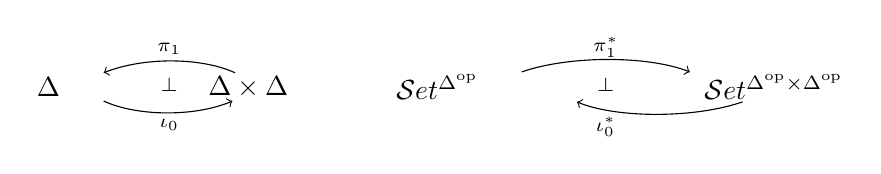
\begin{tikzpicture}[x=1.9em,y=1.5em]
  \node (d)   at (0,0)     {$\Delta$};
  \node (dd)  at (3.8,0)   {$\Delta\times\Delta$};
  \draw[->] (3.55,0.34) .. controls (2.9,0.72) and (1.8,0.72) .. (1.05,0.34);
  \node at (2.3,0.92) {$\scriptstyle\pi_{1}$};
  \node at (2.3,0.05) {$\scriptstyle\bot$};
  \draw[->] (1.05,-0.34) .. controls (1.7,-0.72) and (2.8,-0.72) .. (3.5,-0.34);
  \node at (2.3,-0.92) {$\scriptstyle\iota_{0}$};
  \node at (5.3,0) {$\rightsquigarrow$};
  \node (s)   at (7.4,0)   {$\Set^{\Delta^{\mathrm{op}}}$};
  \node (ss)  at (13.8,0)  {$\Set^{\Delta^{\mathrm{op}}\times\Delta^{\mathrm{op}}}$};
  \draw[->] (9.0,0.36) .. controls (9.9,0.76) and (11.4,0.76) .. (12.2,0.36);
  \node at (10.6,0.96) {$\scriptstyle\pi_{1}^{*}$};
  \node at (10.6,0.05) {$\scriptstyle\bot$};
  \draw[->] (13.2,-0.36) .. controls (12.3,-0.76) and (10.8,-0.76) .. (10.05,-0.36);
  \node at (10.6,-0.96) {$\scriptstyle\iota_{0}^{*}$};
\end{tikzpicture}
\end{rveq}
Joyal 与 Tierney 证明了这一对函子定义拟范畴模型结构与\trCompleteSegalSpaces{}%
模型结构之间的一个 Quillen \trEquivalence{} \cite[4.11]{bib64}。经检视，其%
\trLeftAdjoint{}保持有限\trProduct，于是\cref{cor:cartesian-closed-cosmos}
适用，从而在全子范畴 $\CSS$ 上创造一个\trCartesianClosed{}\trInfinityCosmos{}结构，其细节如\cref{prop:change-of-base-model-cosmoi}所述，
对此 $(\text{--})_{0}\coloneqq\mathrm{row}_{0}=:\ \iota_{0}^{*}$ 是一个%
\trCosmologicalBiequivalence。

第二个介于单纯集与双单纯集之间、方向相反的伴随，其\trLeftAdjoint{}定义为
沿 \trYonedaEmbedding{} $\Delta\times\Delta\hookrightarrow\Set^{\Delta^{\mathrm{op}}\times\Delta^{\mathrm{op}}}$ 对函子
\[
\begin{aligned}
\Delta\times\Delta &\longrightarrow \Set^{\Delta^{\mathrm{op}}}\\
{[m]}\times{[n]} &\longmapsto \Delta[m]\times\qcInt[n]
\end{aligned}
\]
所作的左\trKanExtension；此处 $\qcInt[n]$ 是这样一个\trGroupoid{}的\trNerve：
它恰有 $n+1$ 个对象、且每个 hom-集中恰有一条态射，由自由逆转序数范畴
$\underline{n+1}$ 中的诸态射而得。\trRightAdjoint{}即 (ii) 之陈述中所描述的
那个相应的「$\rvNerve$」函子。Joyal 与 Tierney 还证明了伴随
\begin{center}
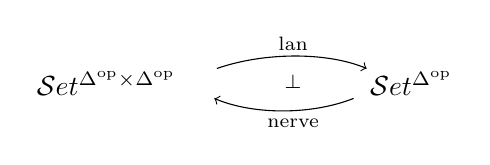
\begin{tikzpicture}[x=1.9em,y=1.5em]
  \node (ss) at (0,0)   {$\Set^{\Delta^{\mathrm{op}}\times\Delta^{\mathrm{op}}}$};
  \node (s)  at (5.8,0) {$\Set^{\Delta^{\mathrm{op}}}$};
  \draw[->] (2.1,0.36) .. controls (3.0,0.76) and (4.2,0.76) .. (4.95,0.36);
  \node at (3.55,0.96) {$\scriptstyle\rvLan$};
  \node at (3.55,0.05) {$\scriptstyle\bot$};
  \draw[->] (4.7,-0.36) .. controls (3.9,-0.76) and (2.8,-0.76) .. (2.05,-0.36);
  \node at (3.55,-0.96) {$\scriptstyle\rvNerve$};
\end{tikzpicture}
\end{center}
相对于\trCompleteSegalSpaces{}与拟范畴的模型结构是一个 Quillen \trEquivalence
\cite[4.12]{bib64}。为了从\cref{cor:right-quillen-adjunction-biequivalence}
得出 $\rvNerve\colon\QCat\to\CSS$ 是一个\trCosmologicalBiequivalence，尚须
证明的只是：这一函子是单纯富集的且保持单纯\trCotensor；或者等价地，由附录 A
中的\cref{prop:enriched-adjoint-preserves-tensors}，伴随
$\rvLan\dashv\rvNerve$ 是单纯富集的。

为验证这一点，我们利用外积\trBifunctor：
\[
\begin{aligned}
\Set^{\Delta^{\mathrm{op}}}\times\Set^{\Delta^{\mathrm{op}}}
&\xrightarrow{\ \square\ }\Set^{\Delta^{\mathrm{op}}\times\Delta^{\mathrm{op}}}\\
(A,\ B) &\longmapsto (A\square B)_{m,n}\coloneqq A_{m}\times B_{n}
\end{aligned}
\]
由于任何双单纯集 $X$ 都可以被复原为诸可表示对象的典范余极限，只需考虑从
可表示双单纯集 $\Delta[m]\square\Delta[n]$ 到单纯集 $A$ 的映射。在刚刚定义
的 $\Set^{\Delta^{\mathrm{op}}\times\Delta^{\mathrm{op}}}$ 之单纯富集中，从
$\Delta[m]\square\Delta[n]$ 到 $\rvNerve(A)$ 的映射单纯集，其 $k$-单纯形定义
为 $\rvNerve(A)^{\Delta[m]\square\Delta[n]}$ 中的 $(k,0)$-单纯形。现在
\[
(\rvNerve(A)^{\Delta[m]\square\Delta[n]})_{k,0}
=\Set^{\Delta^{\mathrm{op}}\times\Delta^{\mathrm{op}}}((\Delta[m]\square\Delta[n])
\times(\Delta[k]\square\Delta[0]),\ \rvNerve(A))
\]
由双单纯集上\trCartesianClosed{}结构的定义而然，而后者
\[
\cong\Set^{\Delta^{\mathrm{op}}\times\Delta^{\mathrm{op}}}((\Delta[m]\times\Delta[k])
\square\Delta[n],\ \rvNerve(A))
\]
由外积的定义而然，后者又
\[
\cong\Set^{\Delta^{\mathrm{op}}}(\rvLan((\Delta[m]\times\Delta[k])\square\Delta[n]),\ A)
\]
由伴随而然。Joyal 与 Tierney 在 \cite[2.11]{bib64} 中证明：左\trKanExtension{}%
作用于外\trTensorProduct{}的方式为 $\rvLan(B\square\Delta[n])\cong B\times\qcInt[n]$。于是我们得到
\[
\begin{aligned}
&\cong\Set^{\Delta^{\mathrm{op}}}((\Delta[m]\times\Delta[k])\times\qcInt[n],\ A)\\
&\cong\Set^{\Delta^{\mathrm{op}}}((\Delta[m]\times\qcInt[n])\times\Delta[k],\ A)\\
&\cong\Set^{\Delta^{\mathrm{op}}}(\rvLan(\Delta[m]\square\Delta[n])\times\Delta[k],\ A)\\
&=:\ (A^{\rvLan(\Delta[m]\square\Delta[n])})_{k}
\end{aligned}
\]
最后一步由单纯集上\trCartesianClosed{}结构的定义而然。这就证明了该伴随与诸
单纯富集相容，于是由\cref{cor:right-quillen-adjunction-biequivalence}与
\cite[4.12]{bib64} 即得：$\rvNerve\colon\QCat\to\CSS$ 是一个%
\trCosmologicalBiequivalence。
\end{proof}

第二种 $(\infty,1)$-\trCategory{}的模型与上述模型密切相关。

\begin{definition}[Segal 范畴]\label{def:segal-categories}
一个\textbf{Segal 前范畴}（Segal precategory）是一个双单纯集
$X_{\bullet}\in\Set^{\Delta^{\mathrm{op}}\times\Delta^{\mathrm{op}}}$，其
$0$-单纯形的空间 $X_{0}$ 在其顶点之集 $X_{0,0}$ 上是 $0$-骨架的。一个%
\textbf{\trSegalCategories{}}是一个 Reedy 纤维性的 Segal 前范畴，%
\footnote{原书此句（A Segal category is a Segal category that is Reedy fibrant and satisfies…）之第二出现疑为「Segal precategory」之误（否则定义
循环），此处径改。——译者注}且满足
\cref{def:complete-segal-space}的 Segal 条件。
\end{definition}

\cref{def:segal-categories}比惯常的定义略强，后者由 Dwyer、Kan 与 Smith
\cite{bib38} 首先引入，又经 Hirschowitz 与 Simpson \cite{bib56} 进一步发展。
惯常的约定定义一个\trSegalCategories{}为一个 Segal 前范畴 $X_{\bullet}$，使
得对每个 $n\ge 2$，由 $n$-\trSimplex{}的\trSpine{}之包含
$\Gamma[n]\hookrightarrow\Delta[n]$ 在加权极限上诱导的映射
\[
X_{n}\cong\operatorname{lim}_{\Delta[n]}X\longrightarrow
X_{1}\times_{X_{0}}\cdots\times_{X_{0}}X_{1}\cong
\operatorname{lim}_{\Gamma[n]}X
\]
\footnote{原书此式末项印作「$\operatorname{lim}_{\Gamma[n]}\Delta[n]$」，疑为
「$\operatorname{lim}_{\Gamma[n]}X$」之误——同式首项作
$\operatorname{lim}_{\Delta[n]}X$，且该映射由 $n$-\trSimplex{}的\trSpine{}之包含
$\Gamma[n]\hookrightarrow\Delta[n]$ 在加权极限上诱导，此处径改。——译者注}
是单纯集之间的一个弱同伦等价——而不要求 Reedy 纤维性。我们更愿意把 Reedy
纤维性纳入我们的\trSegalCategories{}概念之中，使得诸\trSegalCategories{}恰是
Segal 前范畴的\trCategory{} $\PCat$ 上某个适当模型结构中的诸\trFibrant{}对象，
而该模型结构随之产出一个\trInfinityCosmos。在我们引入\trInfinityCosmos{}
$\Segal$ 之前，我们先解释如何把一个\trCompleteSegalSpaces{}变换为一个%
\trSegalCategories。

\begin{lemma}\label{lem:discretization}
存在一个称作\textbf{离散化}（discretization）的函子 $\rvDisc\colon\Set^{\Delta^{\mathrm{op}}\times\Delta^{\mathrm{op}}}\to\Set^{\Delta^{\mathrm{op}}\times\Delta^{\mathrm{op}}}$，由下列\trPullback{}定义%
\footnote{原书本引理中离散化函子之定义域与余定义域两处、以及下文两处%
$\PCat$ 之包含，上标均印作短形 $\Set^{\Delta^{\mathrm{op}}}$；按数学文义
（离散化系双单纯集的自函子，$\PCat$ 系双单纯集之子范畴）均应为%
$\Set^{\Delta^{\mathrm{op}}\times\Delta^{\mathrm{op}}}$，径改。——译者注}
\begin{center}
\begin{tikzpicture}[x=2.1em,y=1.5em]
  \node (dl) at (0,1.5)   {$\rvDisc(X)$};
  \node (tr) at (5.4,1.5) {$X$};
  \node (bl) at (0,0)     {$\mathrm{cosk}_{0}(X_{0,0})$};
  \node (br) at (5.4,0)   {$\mathrm{cosk}_{0}(X_{0})$};
  \draw[right hook->] (dl) -- (tr);
  \draw[right hook->] (bl) -- (br);
  \draw[->] (0,1.15) -- (0,0.35);
  \draw[->] (5.4,1.15) -- (5.4,0.35);
  \node at (0.62,1.12) {$\scriptstyle\lrcorner$};
\end{tikzpicture}
\end{center}
它落入 Segal 前范畴的子范畴之中，而且确为包含 $\PCat\hookrightarrow\Set^{\Delta^{\mathrm{op}}\times\Delta^{\mathrm{op}}}$ 的\trRightAdjoint。
此外，一个 Reedy 纤维性的 Segal 空间之离散化是一个\trSegalCategories。
\end{lemma}

\begin{proof}
由于「顶点求值」映射 $X\to\mathrm{cosk}_{0}(X_{0})$ 在第 $0$ 列上双射，%
\trPullback{} $\rvDisc(X)\to\mathrm{cosk}_{0}(X_{0,0})$ 亦必如此。于是
$\rvDisc(X)_{0}\cong X_{0,0}$，这就证明了 $\rvDisc(X)$ 是一个 Segal 前范畴。
为证明伴随性，注意：对任何 Segal 前范畴 $Y$ 与双单纯映射 $f\colon Y\to X$，
其分量 $f_{0}\colon Y_{0}\to X_{0}$ 由 $Y$ 的离散性唯一地经过
$X_{0,0}\hookrightarrow X_{0}$ 分解。这就诱导出 $f$ 经过 $\rvDisc(X)\hookrightarrow X$ 的所需唯一分解。

最后，任何 $0$-余骨架的单纯空间自动是 Reedy 纤维性的并且是一个 Segal 空间，
因为\cref{def:complete-segal-space}(i) 与 (ii) 的诸映射都是\trIsomorphism。
当 $X$ 是 Reedy 纤维性的时，映射 $X_{n}\to\mathrm{cosk}_{0}(X_{0})_{n}\cong X_{0}^{n}$ 是一个\trKanFibration，于是定义单纯集 $\rvDisc(X)_{n}$ 的那个%
\trPullback{}是一个同伦拉回。将附录 C 中的\cref{lem:pullback-we-between-fibrations}施于单纯集上 Quillen 的 Kan 复形模型结构，$X$ 的诸 Segal 映射
(ii) 经拉回便定义 $\rvDisc(X)$ 的类似的弱同伦等价。
\end{proof}

\begin{proposition}\label{prop:segal-cosmos}
\trSegalCategories{}的全子范畴 $\Segal\hookrightarrow\PCat$ 定义一个%
\trCartesianClosed{}\trInfinityCosmos，其中\trFunctorSpace{} $\Fun(A,B)$
定义为底\trQuasiCategory，它由每个\trInternalHom{} $B^{A}$ 中的顶点构成。
相对于这一\trInfinityCosmos{}结构：
\begin{enumerate}[label=(\roman*)]
\item 底\trQuasiCategory{}\trFunctor{} $(\text{--})_{0}\coloneqq\mathrm{row}_{0}\colon\Segal\rightleftarrows\QCat$ 是一个%
  \trCosmologicalBiequivalence。
\item 存在一个\trCosmologicalBiequivalence{} $\rvDisc\colon\CSS\rightleftarrows\Segal$，
  它把一个\trCompleteSegalSpaces{}「离散化」为一个\trSegalCategories。
\item 另一个\trCosmologicalBiequivalence{} $\rvNerve\colon\QCat\rightleftarrows\Segal$
  把一个\trQuasiCategory{} $A$ 送到这样一个双单纯集，其 $(m,n)$-单纯形是
  单纯映射 $\Delta[m]\times\Delta[n]\to A$，其在 $\Delta[m]$ 的每个顶点处的
  分量均为常值。
\end{enumerate}
\end{proposition}
\begin{proof}
由 Pellissier 与 Bergner \cite{bib90,bib13,bib14}，诸（Reedy 纤维性的）%
\trSegalCategories{}构成承载于 Segal 前范畴的\trCategory{}之上的一个%
\trCartesianClosed{}\trModelStructure{}的诸\trFibrant{}对象，其中一切对象
皆\trCofibrant。$\PCat$ 上的\trCartesianClosed{}结构可以显式定义，或者从
$\PCat$ 是一个预层\trCategory{}这一观察推得（见\cref{ex:pcat-presheaves-quotient}）。

\eqref{eq:pi-iota-adjunction} 的诸伴随函子限制为单纯集与 Segal 前范畴之间的
一个伴随，Joyal 与 Tierney 证明后者定义拟范畴模型结构与\trSegalCategories{}%
模型结构之间的一个 Quillen \trEquivalence{} \cite[5.6]{bib64}。再次经检视，
其\trLeftAdjoint{}保持有限\trProduct，于是\cref{cor:cartesian-closed-cosmos}
适用，从而在全子范畴 $\Segal$ 上创造一个\trCartesianClosed{}\trInfinityCosmos{}结构，对此 $(\text{--})_{0}\coloneqq\mathrm{row}_{0}=:\ \iota_{0}^{*}$ 是一个\trCosmologicalBiequivalence。

由 Bergner 的一条定理，\cref{lem:discretization}的包含$\dashv$离散化伴随定义%
\trCompleteSegalSpaces{}模型结构与\trSegalCategories{}模型结构之间的一个
Quillen \trEquivalence{} \cite[\S6]{bib14}。为了从%
\cref{cor:right-quillen-adjunction-biequivalence}得出 $\rvDisc\colon\CSS\to\Segal$ 是一个\trCosmologicalBiequivalence，尚须证明的只是：这一函子是单纯
富集的且保持单纯\trCotensor；或者等价地，由附录 A 中的%
\cref{prop:enriched-adjoint-preserves-tensors}，该伴随是单纯富集的。这由
下述事实得出：这一伴随与 $\CSS$ 和 $\Segal$ 的底\trQuasiCategory{}伴随交换
（见\cref{rem:disc-commutes}）。特别地，由于包含 $\PCat\hookrightarrow\Set^{\Delta^{\mathrm{op}}\times\Delta^{\mathrm{op}}}$ 保持二元\trProduct，
对任何双单纯集 $C$ 与 Segal 前范畴 $S$，有 $\rvDisc(C^{S})\cong\rvDisc(C)^{S}$。类似的论证表明诸单纯\trCotensor{}被保持。过渡到底%
\trQuasiCategory，这就诱导出所需的单纯富集伴随，它使 $\rvDisc\colon\CSS\to\Segal$ 成为单纯的——从而是\trCosmological。

第二个介于单纯集与 Segal 前范畴之间、方向相反的伴随，其\trLeftAdjoint{}由
沿对角函子 $\Delta\colon\Delta^{\mathrm{op}}\to\Delta^{\mathrm{op}}\times\Delta^{\mathrm{op}}$ 的限制定义，而其\trRightAdjoint{}——我们称作
「$\rvNerve$」——由沿同一函子的右\trKanExtension{}继以离散化给出。Joyal 与
Tierney 还证明了这一伴随相对于\trCompleteSegalSpaces{}与拟范畴的模型结构
定义一个 Quillen \trEquivalence{} \cite[5.7]{bib64}。如上，为了得出
$\rvNerve\colon\QCat\to\Segal$ 是一个\trCosmologicalBiequivalence，尚须
论证的只是：这一伴随是单纯富集的。由于函子 $\rvNerve$ 是对角函子
$\rvDiag\colon\Set^{\Delta^{\mathrm{op}}\times\Delta^{\mathrm{op}}}\to\Set^{\Delta^{\mathrm{op}}}$ 之\trRightAdjoint{}继以离散化的复合，而我们已
论证过后一伴随是单纯富集的，故只需证明 $\rvDiag\dashv\rvRan$ 是单纯富集的。

为此，试考虑一个双单纯集 $X$ 与一个单纯集 $A$。由定义
\[
\begin{aligned}
(\rvRan(A)^{X})_{k}
&\coloneqq(\rvRan(A)^{X})_{k,0}
 \coloneqq\Set^{\Delta^{\mathrm{op}}\times\Delta^{\mathrm{op}}}
 (X\times(\Delta[k]\square\Delta[0]),\ \rvRan(A))\\
&\cong\Set^{\Delta^{\mathrm{op}}}(\rvDiag(X\times(\Delta[k]\square\Delta[0])),\ A)\\
&\cong\Set^{\Delta^{\mathrm{op}}}(\rvDiag(X)\times\Delta[k],\ A)
 =:\ (A^{\rvDiag(X)})_{k},
\end{aligned}
\]
此即所欲证。\footnote{原书两行上标印作
$\Set^{\Delta^{\mathrm{op}}\times\Delta^{\mathrm{op}}}$，按
$\rvDiag\dashv\rvRan$ 之型当作 $\Set^{\Delta^{\mathrm{op}}}$，径改。——译者注}
\end{proof}

\begin{remark}\label{rem:disc-commutes}
这一离散化函子与诸底\trQuasiCategory{}函子交换：
\begin{center}
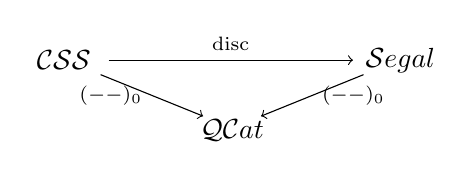
\begin{tikzpicture}[x=1.9em,y=1.5em]
  \node (css)   at (0,1.7)   {$\CSS$};
  \node (segal) at (6.4,1.7) {$\Segal$};
  \node (qcat)  at (3.2,0)   {$\QCat$};
  \draw[->] (0.85,1.7) -- node[above]{$\scriptstyle\rvDisc$} (5.5,1.7);
  \draw[->] (0.7,1.35) -- node[left]{$\scriptstyle(\text{--})_{0}$} (2.65,0.35);
  \draw[->] (5.7,1.35) -- node[right]{$\scriptstyle(\text{--})_{0}$} (3.75,0.35);
\end{tikzpicture}
\end{center}
这最容易通过在模型范畴层面考虑这些函子的\trLeftAdjoint{}而看出。然而，
离散化并不与诸 $\rvNerve$ 构造严格交换，只是在等价意义下交换。对一个%
\trQuasiCategory{} $A$，$\rvNerve(A)$ 是这样一个\trSegalCategories：其
$(m,n)$-单纯形由单纯映射 $\Delta[m]\times\Delta[n]\to A$ 之集给出，这些映射
在 $\Delta[m]$ 的每个顶点处的分量均为常值。相比之下，$\rvDisc(\rvNerve(A))$
是这样一个\trSegalCategories：其 $(m,n)$-单纯形由单纯映射 $\Delta[m]\times\qcInt[n]\to A$ 之集给出，这些映射在 $\Delta[m]$ 的每个顶点处的分量均为
常值。
\end{remark}

从附录 D 中的\cref{dig:saturation-higher-simplices}回忆起：一个 $1$-复状%
\trSimplicialSet{}是一个 $1$-平凡且饱和的复状\trSimplicialSet（见附录 D 中的
\cref{def:complicial-set}、\cref{def:n-trivial}与\cref{def:1-saturated}）。
附录 D 中的\cref{thm:natural-marking-complicial}把诸\trQuasiCategory{}与
$1$-复状\trSimplicialSet——它们在那里被称作「自然标记拟范畴」——等同起来，
因此毫不意外：

\begin{proposition}\label{prop:one-complicial-cosmos}
$1$-复状\trSimplicialSet{}的全子范畴 $\OneComp\hookrightarrow1\text{-}\sSet^{+}$ 定义一个\trCartesianClosed{}\trInfinityCosmos，其中%
\trFunctorSpace{} $\Fun(A,B)$ 定义为\trInternalHom{} $B^{A}$ 的底%
\trQuasiCategory。相对于这一\trInfinityCosmos{}结构，底\trQuasiCategory{}%
\trFunctor{} $(\text{--})_{0}\colon\OneComp\rightleftarrows\QCat$ 与自然标记%
\trFunctor{} $(\text{--})^{\natural}\colon\QCat\rightleftarrows\OneComp$ 都是%
\trCosmological。
\end{proposition}
\begin{proof}
由 Lurie \cite[\S3.1.3--4]{bib78} 与 Verity \cite[\S6.5]{bib129} 各自独立的
定理，诸自然标记拟范畴——我们称之为\textbf{$1$-复状\trSimplicialSet}——
构成承载于\trMarkedSimplicialSet{}的\trCategory{}之上的一个%
\trCartesianClosed{}\trModelStructure{}的诸\trFibrant{}对象，其中一切对象
皆\trCofibrant。存在一个伴随
\begin{center}
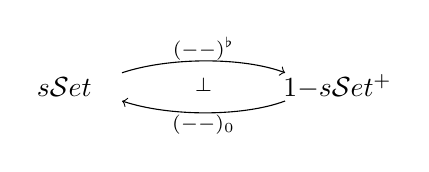
\begin{tikzpicture}[x=1.9em,y=1.5em]
  \node (s) at (0,0)   {$\sSet$};
  \node (c) at (5.2,0) {$1\text{-}\sSet^{+}$};
  \draw[->] (1.1,0.34) .. controls (2.0,0.72) and (3.4,0.72) .. (4.2,0.34);
  \node at (2.65,0.92) {$\scriptstyle(\text{--})^{\flat}$};
  \node at (2.65,0.05) {$\scriptstyle\bot$};
  \draw[->] (4.2,-0.34) .. controls (3.4,-0.72) and (2.0,-0.72) .. (1.1,-0.34);
  \node at (2.65,-0.92) {$\scriptstyle(\text{--})_{0}$};
\end{tikzpicture}
\end{center}
其中\trRightAdjoint{}遗忘标记，而\trLeftAdjoint{}给每个单纯集指派极小
$1$-平凡标记；Lurie 证明了后者是拟范畴模型结构与 $1$-复状\trSimplicialSet{}%
模型结构之间的一个 Quillen \trEquivalence{} \cite[3.1.5.1]{bib78}。经检视，
其\trLeftAdjoint{}保持有限\trProduct，\footnote{注意，作为带标记单纯集，
$(\Delta[1]\times\Delta[1])^{\flat}\ne\Delta[1]^{\flat}\times\Delta[1]^{\flat}$；
因此，有限积保持性质要想成立，极小标记函子落入 $1$-平凡带标记单纯集的%
\trCategory{}之中是本质性的。}于是\cref{cor:cartesian-closed-cosmos}适用，
从而在全子范畴 $\OneComp$ 上创造一个\trCartesianClosed{}\trInfinityCosmos{}结构，使得\trForgetfulFunctor{}定义一个%
\trCosmologicalBiequivalence{} $(\text{--})_{0}\colon\OneComp\rightleftarrows\QCat$，它与底\trQuasiCategory{}\trFunctor{}重合。$1$-复状\trSimplicialSet{}%
的\trModelCategory{}经由此构造而富集于拟范畴模型结构之上，这一事实已在
\cite[3.1.4.5]{bib78} 中被观察到。

对任何拟范畴 $A$ 与 $B$，观察到存在一个自然\trIsomorphism{}
$\Fun(A,B)\cong\Fun(A^{\natural},B^{\natural})$：一侧是 $\QCat$ 中的函子%
\trQuasiCategory，另一侧是刚刚定义的、$\OneComp$ 中介于其自然标记之间的%
\trFunctorSpace；要点在于，单纯映射 $A\to B$ 保持诸\trIsomorphism，从而保持
自然标记。Verity 证明：自然标记函子 $(\text{--})^{\natural}\colon\QCat\to\OneComp$ 创造诸\trFibrant{}对象之间的诸\trFibration{} \cite[114--118]{bib129}。
由于 $\QCat$ 与 $\OneComp$ 中的诸\trLimit{}都在 $s\Set$ 中被创造，由此得出：
函子 $(\text{--})^{\natural}\colon\QCat\to\OneComp$ 是一个%
\trCosmologicalBiequivalence，而且确是 $(\text{--})_{0}\colon\OneComp\to\QCat$
的一个逆\trIsomorphism。
\end{proof}

\subsection*{练习}

\begin{exercise}\label{ex:pcat-presheaves-quotient}
Joyal 与 Tierney 把子范畴 $\PCat\hookrightarrow\Set^{\Delta^{\mathrm{op}}\times\Delta^{\mathrm{op}}}$ 等同于由 $\Delta\times\Delta$ 的 $1$-范畴性商
$\Delta\vert_{2}$ 所索引的预层\trCategory，这一商由逆转函子
$[0]\times\Delta\hookrightarrow\Delta\times\Delta$ 像中的诸映射而定义
\cite[5.4]{bib64}。从这一观点出发，重新定义\cref{prop:segal-cosmos}之证明中
出现的、介于 $\PCat$、$\Set^{\Delta^{\mathrm{op}}\times\Delta^{\mathrm{op}}}$
与 $\Set^{\Delta^{\mathrm{op}}}$ 之间的三个伴随。
\end{exercise}

\begin{exercise}\label{ex:nerve-sections}
验证：诸\trCosmologicalBiequivalence{} $\rvNerve\colon\QCat\rightleftarrows\CSS$
与 $\rvNerve\colon\QCat\rightleftarrows\Segal$ 各自定义相应底%
\trQuasiCategory{}函子的一个\trSection。
\end{exercise}

